\chapter{Genome assembly and characterization}
\section{Introduction}
Ascidians are marine invertebrates that spend their adult life filter feeding through an incurrent siphon and an outcurrent siphon. Ascidians are evolutionarily interesting because of the phylogentic position\textemdash urochordates\textemdash the sister group to vertebrates and cephalochordates, together they form the chordate phylum. Although ascidans share no resemblance to vertebrates in their adult stage, they share several features, a notochord, dorsal hollow neural tube, and gill slits during development in addition to 18S placement (wada and satoh, 1994, Cameron et al 2000). The development of ascidians are well documented, the cell lineage from fertilization to gastrulation has be followed in \textit{Ciona intestinalis} \cite{nishida_cell_1983,nishida_cell_1985,nishida_cell_1987}. Studies of other ascidians species have shown that the majority of phyla has an invariant cell lineage and typical development \cite{berrill_studies_1931}. Only very few solitary ascidians have deviated and undergone tail-loss \cite{swalla_interspecific_1990, tsagkogeorga_updated_2009}. \textit{M. occulta} and \textit{M. oculata} are two species that are found in the shallow waters for Roscoff, France that closely resemble each other in their adult stage, they differ only by a white pigment spot found between the siphons of \textit{M. oculata} Figure~\ref{fig:adults}. These two text it{Molgula} species, however, have different methods of development\textemdash \textit{M. oculata} developing a typical tadpole larvae and \textit{M. occulta} developing without a tail. Many of the genes have been studied across a number of ascidian, showing that gene function tends to be orthologous within the phyla \cite{satoh_ascidian_2003}. 

although genes tend to be expressed in homolguous patterns and tissues, the presence of gens are not the same across species . there has also been cases where genes that have been shown to be important for important biological process are absence in spies why the affected phonotype. it has also been shown that in ascidians with the same phenotype and gene expression, regulatory modules are not necessarily the same. Ascidian speices are far more divergent than the appear phenotypicaly. Genomics has shed some light on the area. because ascidians are board cast spawners they are highly polymorhpic and has rapid rates of evolution. this has cause fairly divergence genomes outside of coding regions. we will demonstrate this using closely related speices and more divergent M. occidentalis. whole genome sequencing and assembly has given us a better picture of what is going on evolutionary for close and divergent species. we are about to charaterize gene networks, identify regulatory elements and get a better understanding of something that sounds really important. here we use next-generation sequencing to compare the genomes of three molgula spp and to charaterize the hox clusters of those spp.

However, as with most biological processes there is  there are cases where gene expression differences led to variation, in addition to genes with important functions . Genomics allows us to identify elements involved in the 
regulation of genes. To identify elements of such, information for a number of species 

Ciona intestinalis was the first ascidian species to be sequenced

\begin{figure}[tbp]
\centering
\includegraphics[scale=0.5]{figures/adults.pdf}
\caption{\textbf{Adult ascidians.} \textit{M. occulta} (A) and \textit{M. oculata} (B) are nearly identical in their adult stage with the white pigment spot (red arrow). Their tunic is covered in sand, seeing that they are found on the sandy sea bottoms. Under there sand covered tunic, the two species differ by the color of their eggs\textemdash purple in \textit{M. oculata}, pictured and an orange-yellowish color in \textit{M. occulta}\textemdash found just above the kidney complex (C). \textit{C. intestinalis} (D) is one of the more studies ascidians and has a assembled genome.}
\label{fig:adults}
\end{figure}

\section{Materials and methods}

\subsection{Genomic DNA library preparation and sequencing}
Genomic DNA was phenol/chloroform extracted from dissected gonads of \textit{Molgula occulta} (Kupffer) and \textit{Molgula oculata} (Forbes) adults from Roscoff, France, and a \textit{Molgula occidentalis} (Traustedt) adult from Panacea, Florida, USA (Gulf Specimen Marine Lab). Genomic DNA was sheared using an M220 Focused-ultrasonicator (Covaris, Woburn, MA). Sequencing libraries were prepared using KAPA HiFi Library Preparation Kit (KAPA Biosystems, Wilmington, MA) indexed with DNA barcoded adapters (BioO, Austin, TX). Size selection was performed using Agencourt (Beckman-Coulter, Brea, CA) AMPure XP purification beads (300-400 bp fragments), or Sage Science (Beverly, MA) Pippin Prep (650-750 bp and 875-975 bp fragments). For \textit{M. occulta} and \textit{M. occidentalis} libraries, 6 PCR cycles were used. For \textit{M. oculata} libraries, 8 cycles were used for the 300-400 bp library, and 10 cycles were used for the 650-750 and 875-975 bp libraries. Libraries of different species but same insert size ranges were multiplexed for sequencing in three 100 � 100 PE lanes on a HiSeq 2000 sequencing system (Illumina, San Diego, CA) at the Genomics Sequencing Core Facility, Center for Genomics and Systems Biology at New York University (New York, NY). Thus, each lane was dedicated to a mix of species, specifically barcoded libraries of a given insert size range. Raw sequencing reads were deposited as a BioProject at NCBI under the ID\# PRJNA253689.
\subsection{Genome sequence assembly}
All genomes were assembled on Michigan State University High Performance Computing Cluster (http://contact.icer.msu.edu). Prior to assembly, read quality was examined using FastQC v0.10.1. Reads were then quality trimmed on both the 5' and 3' end using seqtk trimfq (https://github.com/lh3/seqtk) which uses Phred algorithm to determine the quality of a given base pair. Seqtk trimfq only trims bases, so no reads were discarded. Each library per species was then abundance filtered using 3-pass digital normalization to remove repetitive and erroneous reads \cite{brown_reference-free_2012,schwarz_genome_2013}, Howe et al., 2014). Genome assembly was done using velvet v1.2.08 \cite{zerbino_velvet:_2008} with k-mer overlap length (`k') ranging from 19 to 69 and scaffolding was done by Velvet, by default. Velvet does not produce separate files for contigs and scaffolds; because Velvet scaffolded conservatively, contigs dominated the assemblies so we refer to both contigs and scaffolds as contigs. CEGMA scores were then computed to evaluate genome completeness \cite{parra_cegma:_2007}. The latest versions of three species' genome assemblies have been deposited on the ANISEED (Ascidian Network for In Situ Expression and Embryological Data) database for browsing and BLAST searching at http://www.aniseed.cnrs.fr/ \cite{tassy_aniseed_2010}. Scripts for genome assembly and CEGMA analysis can be found in the following github repository: https://github.com/elijahlowe/molgula\textunderscore genome\textunderscore assemblies.git
\subsection{Gene identification and alignments}
Thirty-nine hox genes were identified in hunman and downloaded from the NCBI database. These sequences were then BLAST against each of the three assembled \textit{Molgula} genomes. The alignments were then extracted BLAST against the NCBI non-redundant database. \textit{Molgula} alignments sequences were extracted, annotated and placed in the following files, mocc\_hox\_aa.fa, mocu\_hox\_aa.fa, and moxi\_hox\_aa.fa, which are located ???. Hox1-13 sequences for human, fruit fly, and Amphioxus were download from `Homeobox Database' (http://homeodb.zoo.ox.ac.uk/). These sequences were then joined with the identified Molgula \textit{hox} genes and used to produce a phylogenetic trees using MAFFT version 7 online rough tree program at http://mafft.cbrc.jp/alignment/server/clustering.html \cite{}.  Additional alignments between the three species were conducted using mVista \cite {} with \textit{M. oculata} as the anchoring sequence because it shows the most similarity between the three \textit{Molgula} species. The LAGAN alignment algorithm was used with translated anchoring to improve alignment because of evolutionary distances\cite{}.    

\section{Results}
\subsection{Genome assemblies assessment}
Genomes of three Molgula species (\textit{M. occidentalis}, \textit{M. oculata}, and \textit{M. occulta}) were sequenced using next-generation sequencing technology and assembled. A common metric for judging the quality of a genome assembly is the contig N50 length, which is determined such that 50\% of the assembly is contained in contigs of this length or greater. We used the contig N50 length to select the best assembly for each species given the varying `k' parameter (length of k-mer overlap). A `k' of 39 yields the best assembly for both \textit{M. occidentalis} and \textit{M. occulta}. The best `k' for \textit{M. oculata} was 61. \textit{M. occidentalis}, \textit{M. occulta}, and \textit{M. oculata} N50 lengths were approximately 26.3 kb, 13 kb, and 34 kb, respectively (Table 1).
\begin{table}[tbp]
\centering
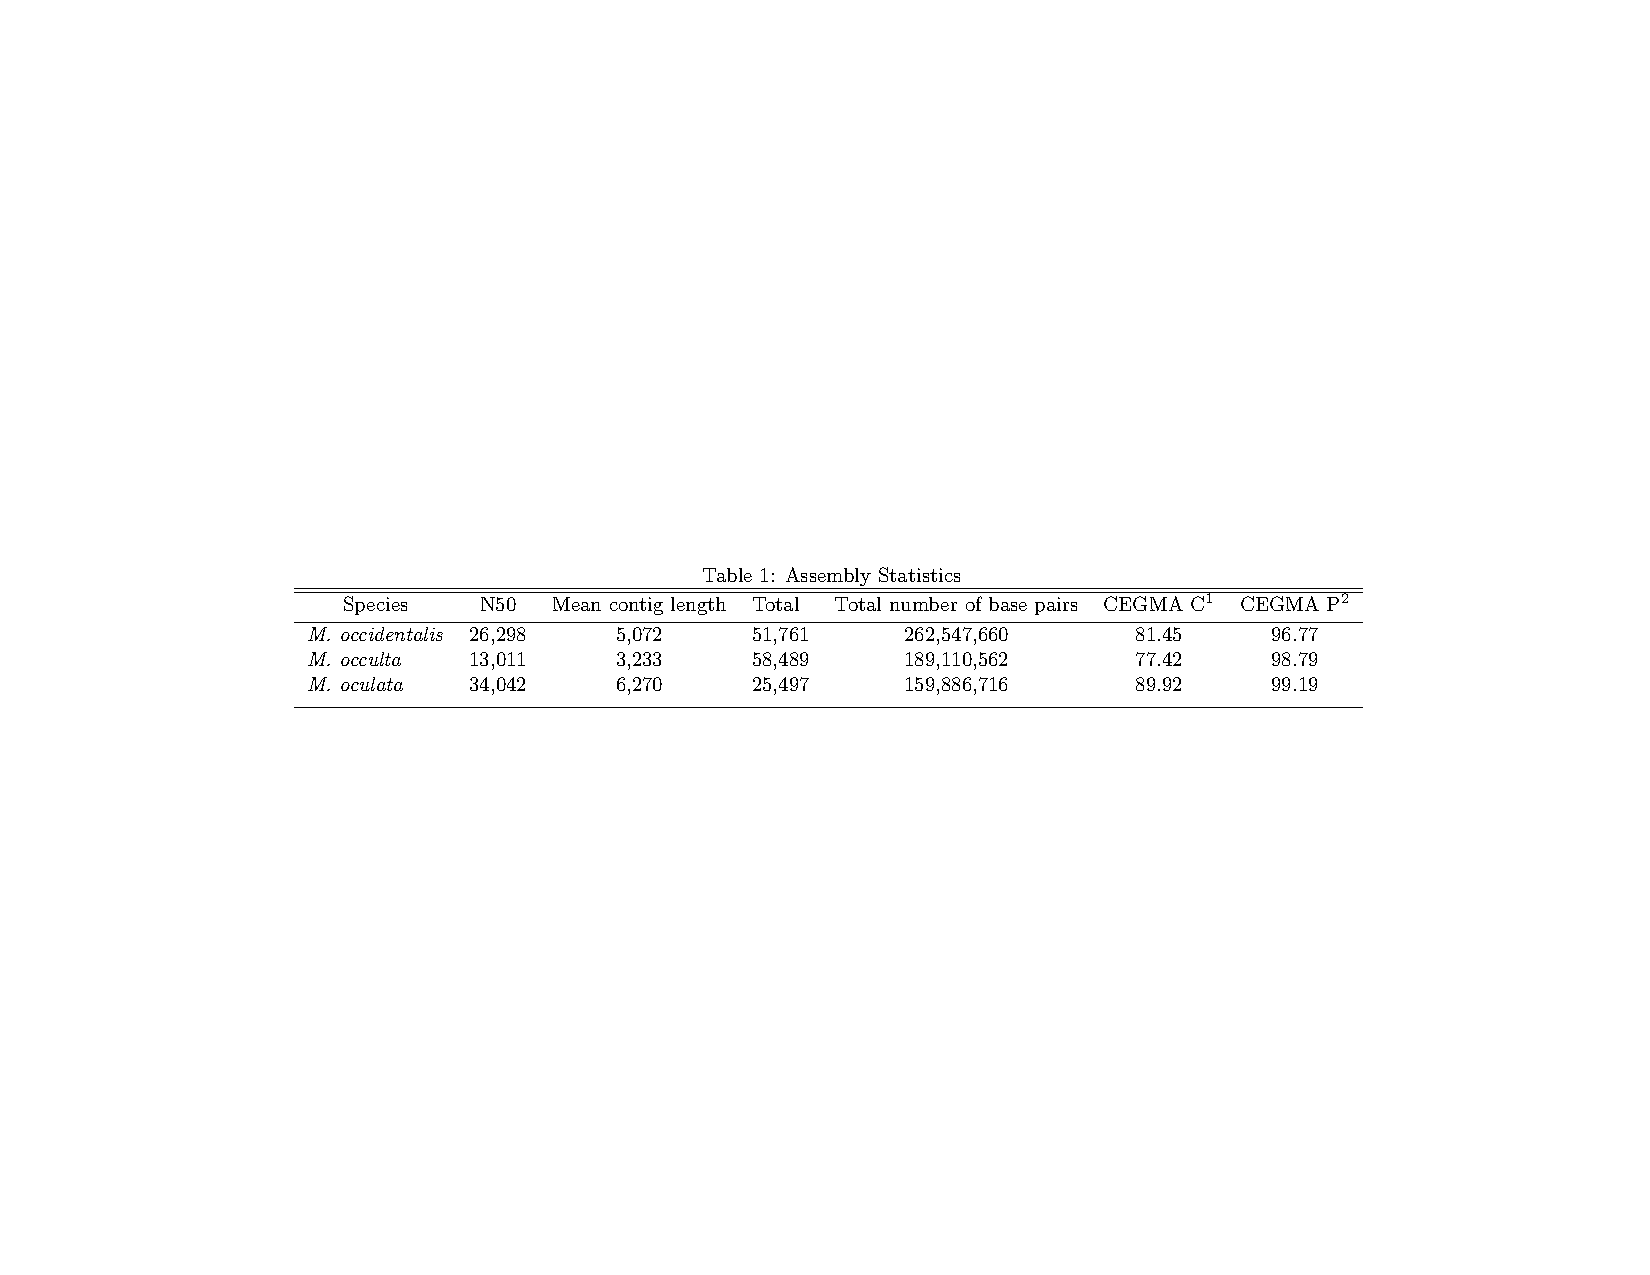
\includegraphics[width=\linewidth]{figures/genome_table_1}
\caption{\textbf{Digitally normalized reads.} The number of reads sequenced before and after digital normalization are shown for each lane of sequencing. The percentage of total reads kept after digital normalization is shown in bold. \textit{M. occulta} had approximately \mytilde237 million reads and was reduced to 91 million reads, a 60\% reduction. \textit{M. oculata} had 150 million reads and reduced by 77\% to \mytilde50 million reads. }
\label{table:genome_table}
\end{table}
In addition to N50 lengths, we also used CEGMA (Core Eukaryotic Genes Mapping Approach) scores, in order to evaluate the assemblies' representative completeness (Parra et al., 2007). CEMGA reports scores for complete and partial alignments to a subset of core eukaryotic genes. An alignment is considered ``complete'' if at least 70\% of a given protein model aligns to a contig in the assembly, while a partial alignment indicates that a statistically significant portion of the protein model aligns. The partial alignment scores are \mytilde97\% or higher for all assemblies. \textit{M. oculata} has the best complete alignment score at \mytilde90\%. \textit{M. occidentalis} and \textit{M. occulta} have complete alignment scores of 81\% and 77\% respectively (Table 1). These scores indicate that our assemblies contain at least partial sequences for the vast majority of protein-coding genes in the genomes of these species.
Various factors make it unreliable to predict genome size and gene density based on assembly metrics alone (Bradnam et al., 2013). Of the handful of sequences we isolated and analyzed, we found that the sizes of introns and upstream regulatory regions were roughly comparable to those from their \textit{Ciona} orthologs. This suggests that the \textit{Molgula} genomes may be as compact as the \textit{C. intestinalis} genome (i.e., \mytilde150-170 Mb, \mytilde16,000 genes, Laird, 1971; Simmen et al., 1998; Satou et al., 2008).
\subsection{Divergence of GRN}
Our sequencing efforts revealed extreme genetic divergence not only between \textit{Ciona} and \textit{Molgula}, as expected, but even within the Molgulids. For example, we used BLAST to identify the \textit{Molgula} orthologs of \textit{C. intestinalis Mesp} (\textit{Ciinte.Mesp}, as per the proposed tunicate gene nomenclature rules, see Stolfi et al., 2014). \textit{Ciinte.Mesp} is the sole ortholog of vertebrate genes coding for \textit{MesP} and \textit{Mesogenin bHLH} transcription factor family members (Satou et al., 2004). VISTA alignment shows high sequence similarity between sequences 5' upstream of the \textit{Mesp} genes from the closely related \textit{M. oculata} and \textit{M. occulta} (Figure 1B). However, there is no conservation of \textit{Mesp} DNA sequences, coding or non-coding, between \textit{M. oculata}/\textit{occulta} and \textit{M. occidentalis}, nor between \textit{C. intestinalis} and any of the three \textit{Molgula} species (Figure 1?figure supplement 1). In previous phylogenetic surveys, \textit{M. occidentalis} has been placed as an early-branching \textit{Molgula} species, often grouped together in a subfamily with species ascribed to the genera Eugyra and Bostrichobranchus instead (Hadfield et al., 1995; Huber et al., 2000; Tsagkogeorga et al., 2009). Our sequencing results support the view that \textit{M. occidentalis} is highly diverged from other \textit{Molgula} spp.

\begin{figure}[tbp]
\centering
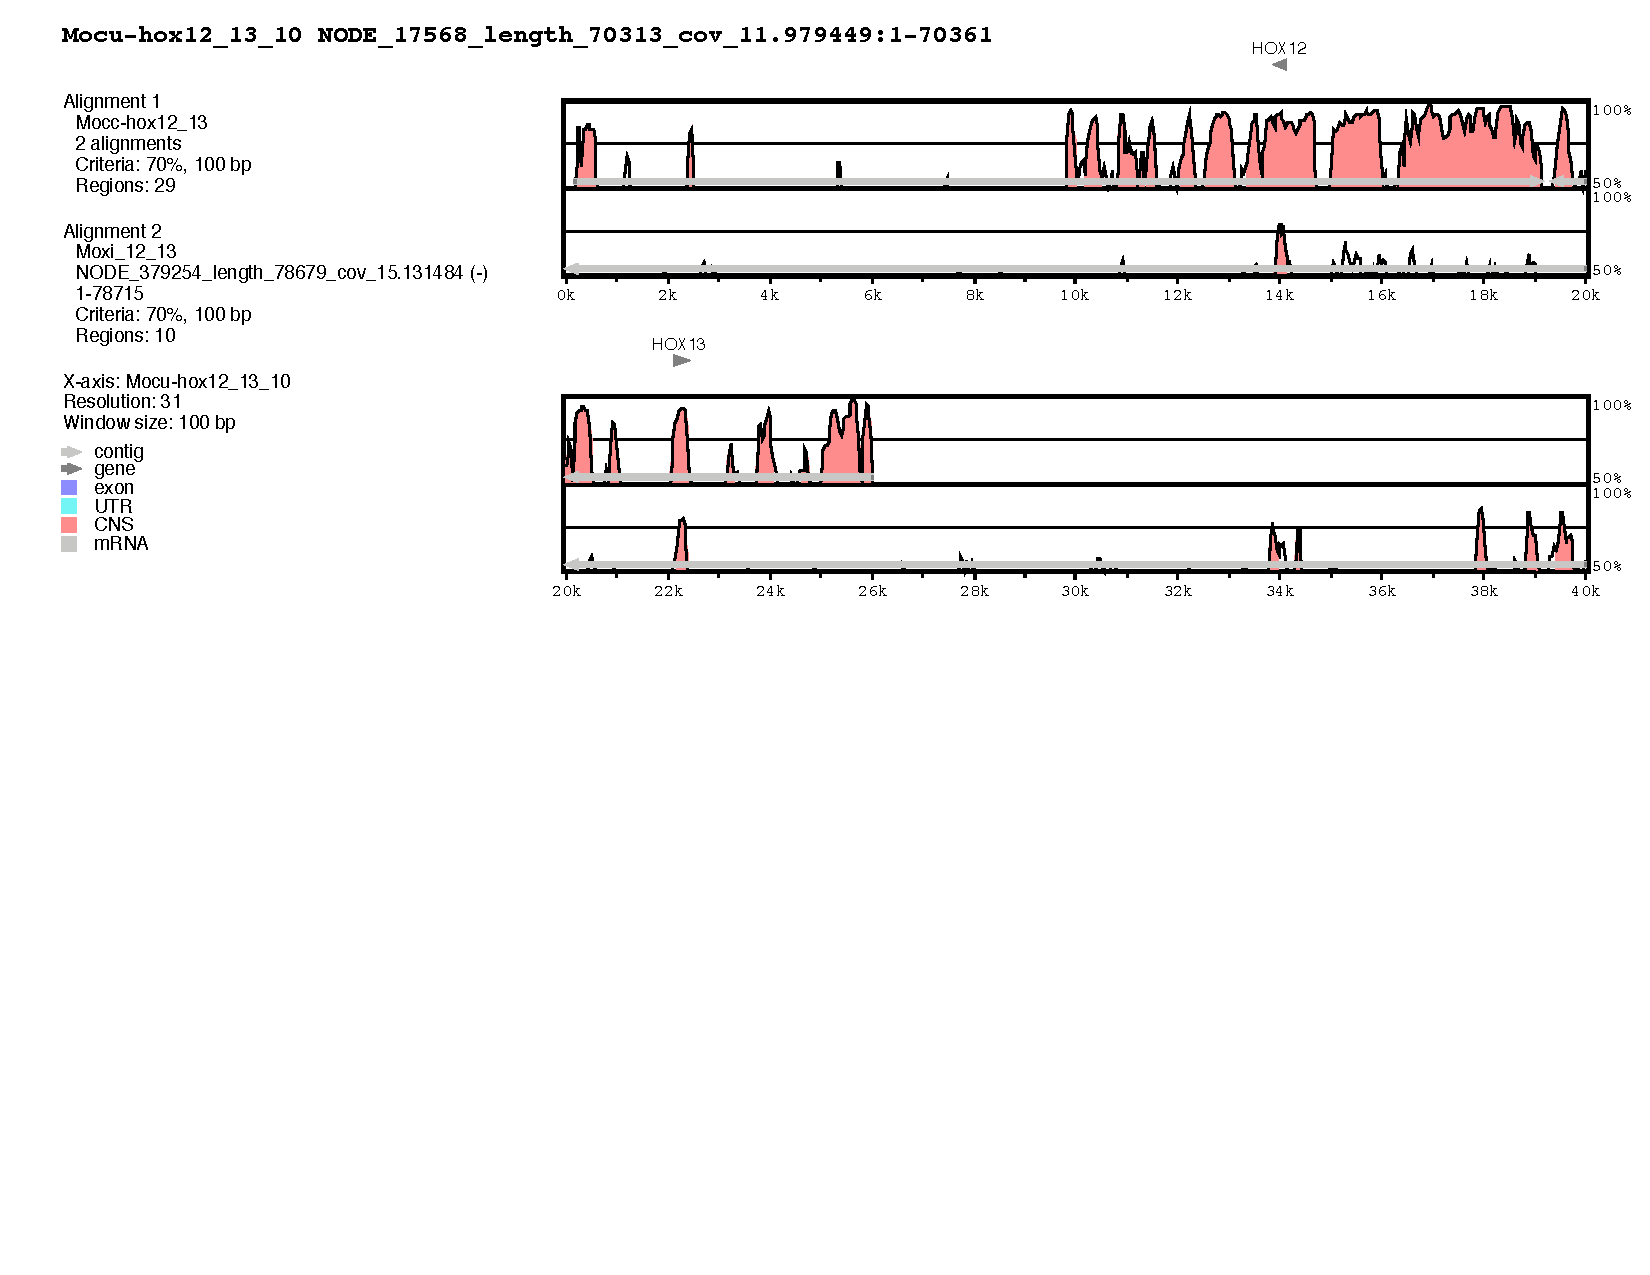
\includegraphics[scale=0.55]{figures/Hox12_13.pdf}
\caption{\textbf{Hox cluster for \textit{Hox 10, 12-13} in \textit{M. occulta}, \textit{M. oculata} and \textit{M. occidentalis}} }
\label{fig:hox12}
\end{figure}
\subsection{Gene complexes}
When studying development it is important to characterize the genome for particular gene cluster/families. There are 4 HOX clusters, in humans  totaling in 39 genes. Ciona has be found to have 9 box genes, Hox1-6, Hox10, and Hox12-13 \cite{Dehal}. Ciona is known to have to two clusters of hox genes across two chromosomes \cite{Ikuta 2004}. Od also has 9 hox genes, hox1-2, hox4, a duplicate hox9, and hox10-13. Eight hox genes have be found in M. occulta and M. oculata, and nine have been found in M. occidentalis. Hox1, hox2, hox3-4, hox5, and hox12-13-10, with hox3-4 being found on the same contig in for both species. Additionally hox10, and hox12-13 are found on the same contig in M. oculata. However, it appears that the hox genes have been rearranged and hox10 is downstream of hox12-13. Hox12-13 are not found on the same contig in M. occulta, however when aligned with mVista there appears to be a strong case for synteny. The same set of hox genes were found in M. occidentalis, hox1-5, hox10 and hox12-13, however, there appears to be a duplicate hox10 gene \mytilde12kb apart found on the same contig. M. occidentalis hox genes span across 5 contigs, hox2 has a stop codon located in the 3-4 helix. 

There is very little synteny between M. occulta, M. oculata and M. occidentalis. When looking at the hox complex for both hox3-4 and hox12-13, only in coding regions does there appear to be syntyany.  

Ciona exhibits longer and than usual introns between hox genes, averaging in the 5Mb range, when typically the hox genes have 100-120 kb separating them \cite{McGinnis 1992}
Because of the lack of homology outside of coding regions, we were able to identify distaless location downstream of hox13 in both M. occidentalis and M. oculata, this was not the case for M. occulta. 
\begin{figure}[tbp]
\centering
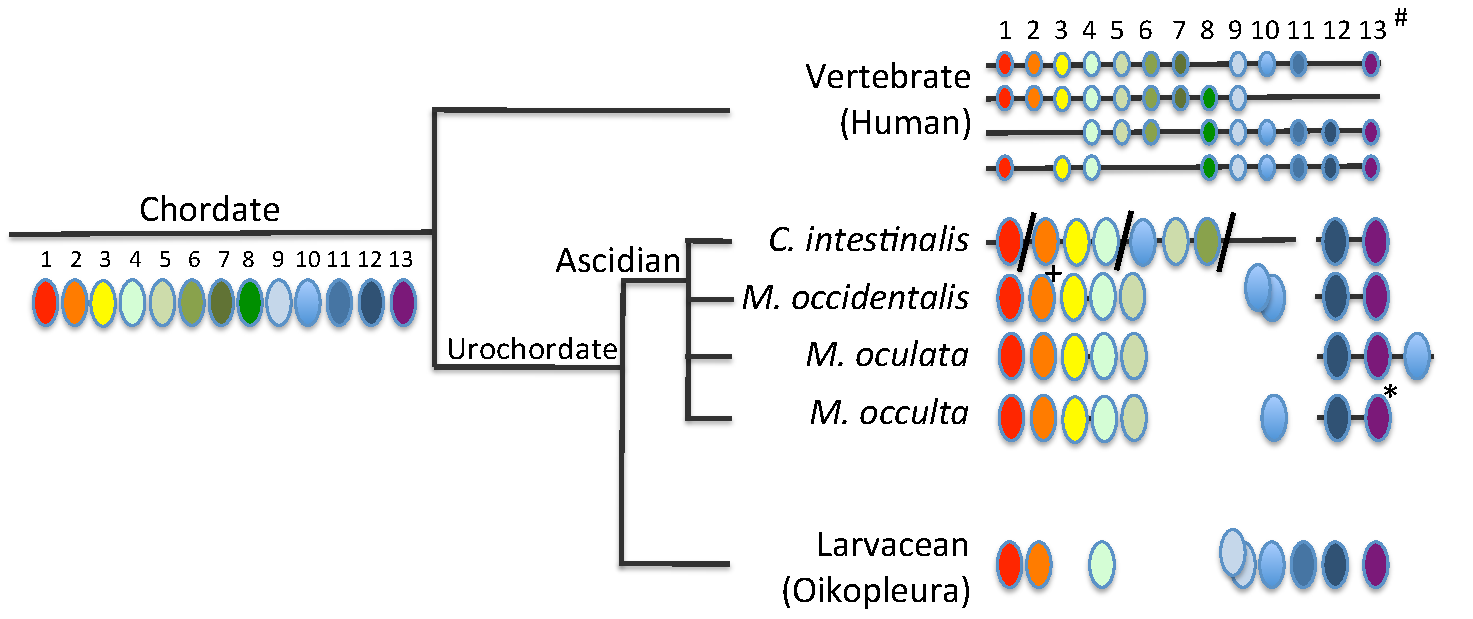
\includegraphics[scale=0.65]{figures/hox.pdf}
\caption{\textbf{Hox cluster for \textit{Hox 10, 12-13} in \textit{M. occulta}, \textit{M. oculata} and \textit{M. occidentalis}} }
\label{fig:hox12}
\end{figure}

\section{Discussion and Conculsion}
Three molgula species have been sequenced and assembled, this is the first of any molgulides to have genomes. 